\documentclass[aspectratio=169,10pt]{beamer}
\usepackage[T1]{fontenc}
\usepackage{lmodern}
\usepackage{amsmath,amssymb}
\usepackage{booktabs}
\usepackage{graphicx}
\usepackage{tikz}
\usetikzlibrary{arrows.meta,positioning,calc,fit,backgrounds}
\graphicspath{{figures/}}

% ------------------------------------------------------------------ look
\definecolor{ink}{HTML}{1B1F24}
\definecolor{accent}{HTML}{0B5CAD}
\definecolor{muted}{HTML}{57606A}
\definecolor{pale}{HTML}{EEF4FB}
\definecolor{okgreen}{HTML}{2E8B57}
\definecolor{warn}{HTML}{C0392B}
\usefonttheme{professionalfonts}
\renewcommand{\familydefault}{\sfdefault}
\setbeamersize{text margin left=0.55cm,text margin right=0.55cm}
\setbeamertemplate{navigation symbols}{}
\setbeamercolor{normal text}{fg=ink}
\setbeamercolor{itemize item}{fg=accent}
\setbeamercolor{enumerate item}{fg=accent}
\setbeamertemplate{itemize item}{\scriptsize$\blacktriangleright$}
\setbeamertemplate{itemize subitem}{\tiny$\bullet$}
\setlength{\leftmargini}{1.1em}
\setbeamertemplate{frametitle}{\vspace*{0.22cm}{\large\bfseries\color{ink}\insertframetitle}\par\vspace{0.03cm}{\color{accent}\rule{1.3cm}{1.6pt}}\vspace{-0.1cm}}
\setbeamertemplate{footline}{\hfill{\tiny\color{muted}\insertframenumber}\hspace{0.3cm}\vspace{0.15cm}}
\newcommand{\takeaway}[1]{\par\vfill\noindent
  \begin{tikzpicture}\node[fill=pale,draw=accent,line width=0.5pt,rounded corners=2pt,text width=\dimexpr\linewidth-10pt\relax,
  inner sep=4pt,align=left]{\footnotesize\textbf{\color{accent}Takeaway.} #1};\end{tikzpicture}\vspace{0.05cm}}
\newcommand{\figcap}[1]{{\tiny\color{muted}#1\par}}
\tikzset{
  box/.style={draw=accent,fill=white,rounded corners=2pt,align=center,font=\scriptsize,minimum height=0.62cm,
              inner sep=2.5pt,line width=0.5pt},
  hbox/.style={box,fill=pale},
  arr/.style={-{Stealth[length=1.6mm]},line width=0.5pt,color=muted},
  note/.style={font=\tiny,color=muted,align=center}}

\begin{document}

% ================================================================== 1 title
\begin{frame}[plain]
\vspace{0.4cm}
\begin{columns}[c]
\column{0.44\textwidth}
{\LARGE\bfseries\color{ink}Autonomous Force-Controlled Surface Treatment with a Legged Mobile Manipulator\par}
\vspace{0.35cm}
{\small\color{muted}Unitree Go2 + Z1 arm, simulated in MuJoCo\par}
\vspace{0.25cm}
\begin{itemize}\small
\item contact surface work: grinding, sanding, coating, inspection
\item curved industrial surfaces behind stairs
\end{itemize}
\column{0.54\textwidth}
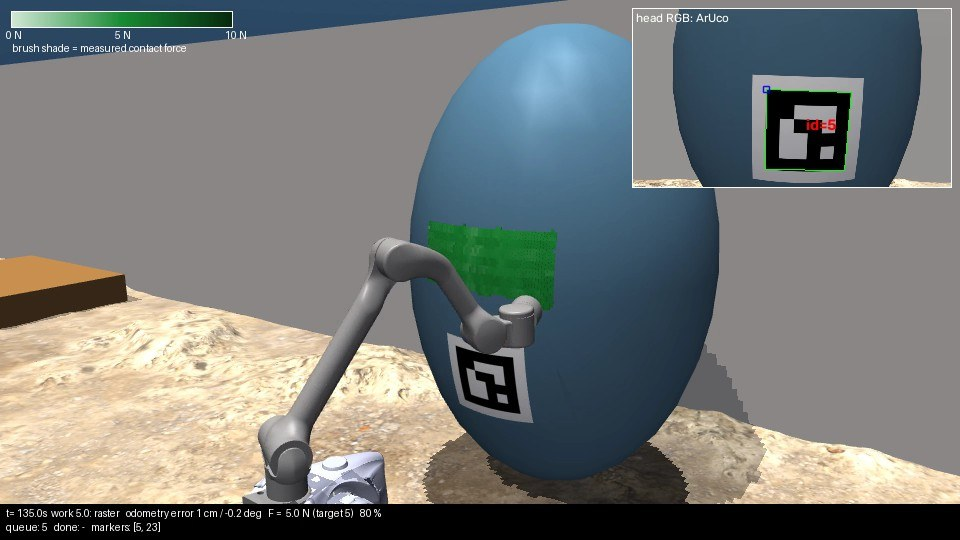
\includegraphics[width=\textwidth]{final_vessel.jpg}\\[1pt]
\figcap{Vessel work order traced at 5\,N; shade = measured force; inset = head camera with the marker.}
\end{columns}
\takeaway{A robot dog that finds its job, walks there and presses on curved surfaces with a controlled force.}
\end{frame}

% ================================================================== 2 why
\begin{frame}{Why does surface work need legs and an arm?}
\begin{columns}[t]
\column{0.42\textwidth}
\begin{itemize}\small
\item Tanks, pipes, hulls sit behind \textbf{stairs}, in tight corridors, on uneven floors
\item Surfaces are \textbf{curved}: the tool must stay normal to them
\item The task is \textbf{contact}: a steady force, not only a position
\end{itemize}
{\tiny\color{muted}qualitative comparison}\\[1pt]
\scriptsize
\begin{tabular}{@{}lcccc@{}}\toprule
 & stairs & reach & force & mobile\\\midrule
wheeled base + arm & \color{warn}$\times$ & \color{okgreen}\checkmark & \color{okgreen}\checkmark & \color{okgreen}\checkmark\\
fixed arm & \color{warn}$\times$ & \color{okgreen}\checkmark & \color{okgreen}\checkmark & \color{warn}$\times$\\
legs only & \color{okgreen}\checkmark & \color{warn}$\times$ & \color{warn}$\times$ & \color{okgreen}\checkmark\\
\textbf{legs + arm} & \color{okgreen}\checkmark & \color{okgreen}\checkmark & \color{okgreen}\checkmark & \color{okgreen}\checkmark\\\bottomrule
\end{tabular}
\column{0.55\textwidth}
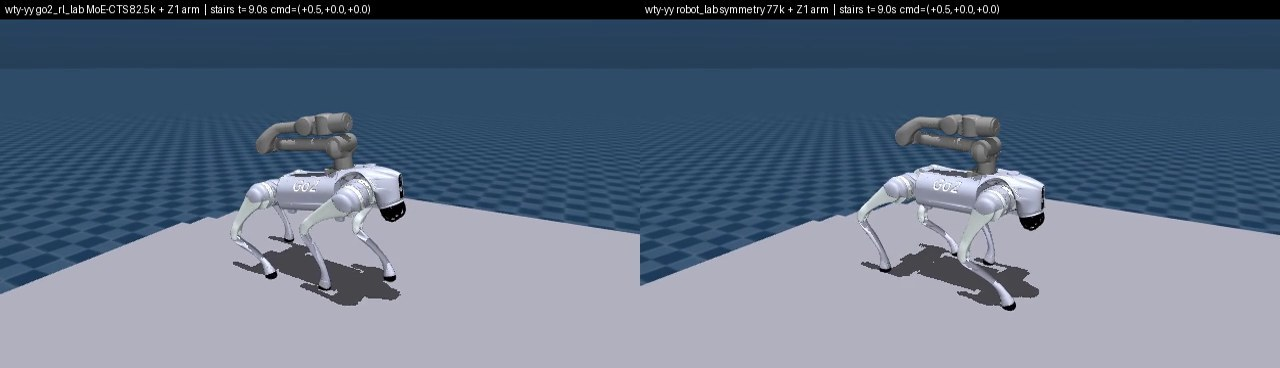
\includegraphics[width=0.9\textwidth]{go2_stairs_arm.jpg}\\[2pt]
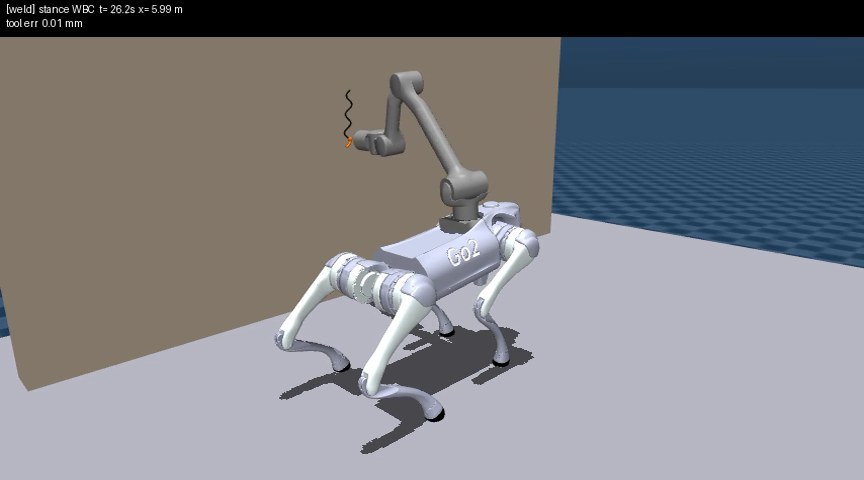
\includegraphics[width=0.45\textwidth]{mission_wallcrack.jpg}\\[1pt]
\figcap{Go2 climbing 10\,cm stairs with the arm on board (top); arm work at a wall beside a stair platform (bottom).}
\end{columns}
\takeaway{Wheels cannot get there and fixed arms cannot move: the robot has to walk \emph{and} work.}
\end{frame}

% ================================================================== 3 task
\begin{frame}{The task: work orders on surfaces the robot has never seen}
\begin{columns}[t]
\column{0.36\textwidth}
\small
\textbf{Given}: a 2-D map (walls, stairs, obstacles); work orders ``cover $W\times H$ next to marker $k$''\\[5pt]
\textbf{Unknown}: where the markers are; the surface geometry; its own exact pose (odometry drifts)\\[5pt]
\textbf{Objective}: cover every area at $F^\ast = 5$\,N along the surface normal
\column{0.62\textwidth}
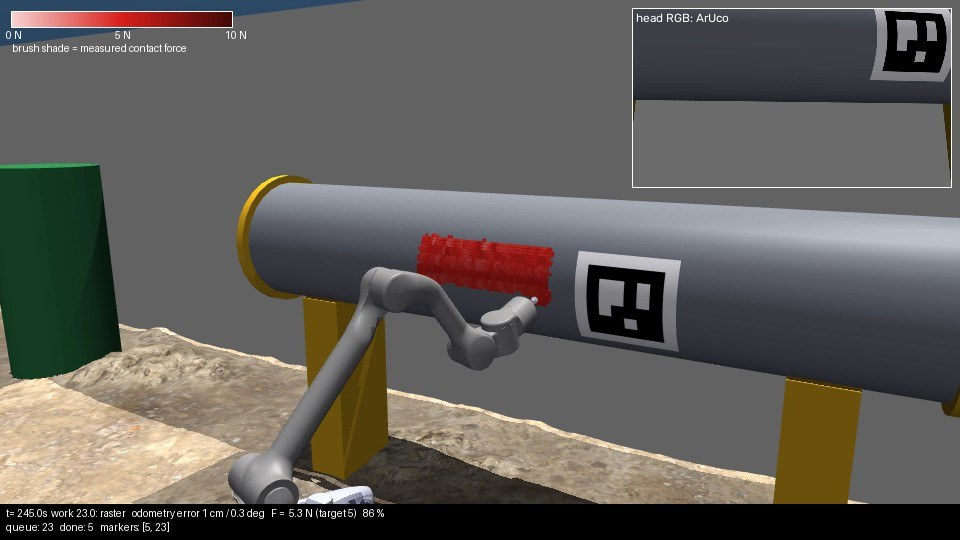
\includegraphics[width=0.49\textwidth]{final_pipe.jpg}\hfill
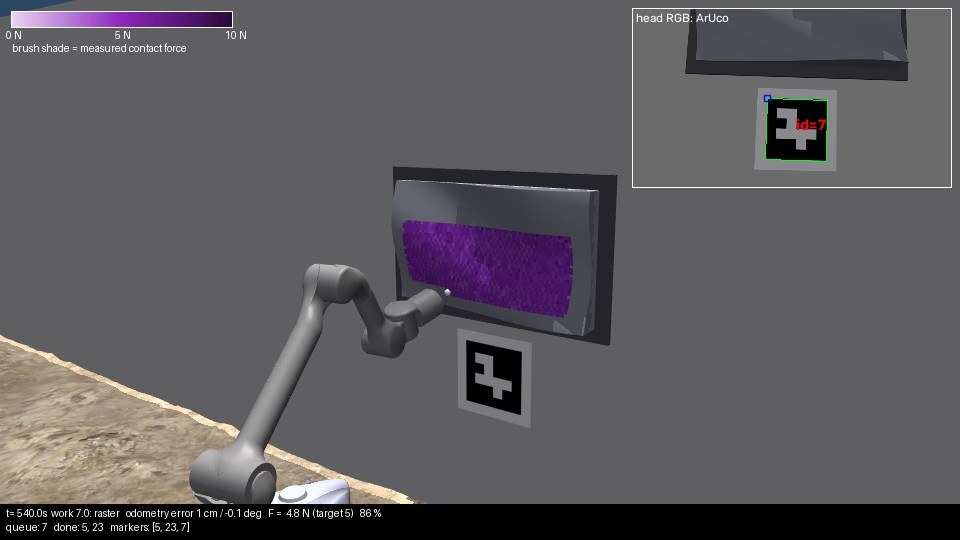
\includegraphics[width=0.49\textwidth]{final_panel.jpg}\\[2pt]
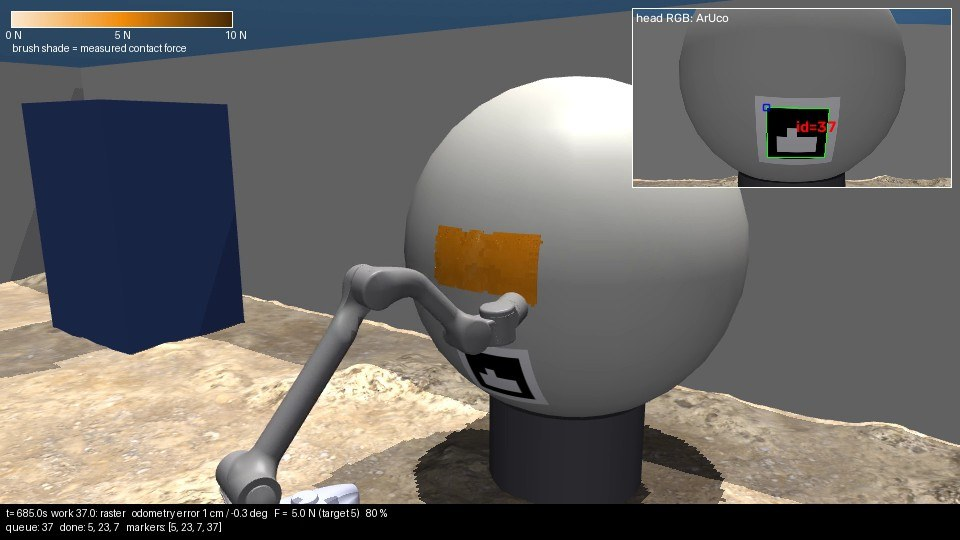
\includegraphics[width=0.49\textwidth]{final_tank.jpg}\hfill
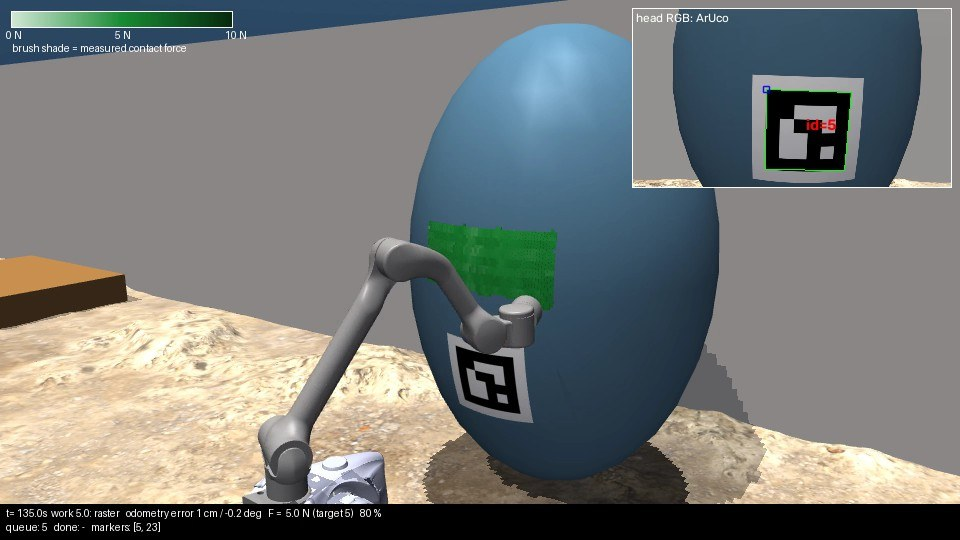
\includegraphics[width=0.49\textwidth]{final_vessel.jpg}\\[1pt]
\figcap{Four surfaces, one ArUco sticker each: horizontal pipe, wavy panel, sphere tank, vessel.}
\end{columns}
\takeaway{The robot never gets the shape of the surface: it has to find and measure every one itself.}
\end{frame}

% ================================================================== 4 architecture
\begin{frame}{How the robot thinks: five layers, one job pipeline}
\centering
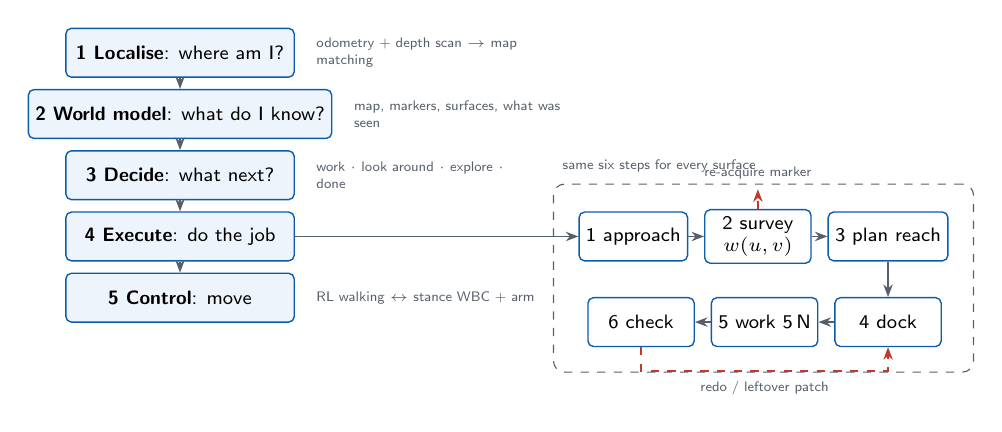
\begin{tikzpicture}[node distance=0.14cm]
\node[hbox,minimum width=2.9cm] (L1) {\textbf{1 Localise}: where am I?};
\node[hbox,minimum width=2.9cm,below=of L1] (L2) {\textbf{2 World model}: what do I know?};
\node[hbox,minimum width=2.9cm,below=of L2] (L3) {\textbf{3 Decide}: what next?};
\node[hbox,minimum width=2.9cm,below=of L3] (L4) {\textbf{4 Execute}: do the job};
\node[hbox,minimum width=2.9cm,below=of L4] (L5) {\textbf{5 Control}: move};
\node[note,right=0.15cm of L1,text width=2.8cm,align=left] {odometry + depth scan $\rightarrow$ map matching};
\node[note,right=0.15cm of L2,text width=2.8cm,align=left] {map, markers, surfaces, what was seen};
\node[note,right=0.15cm of L3,text width=2.8cm,align=left] {work $\cdot$ look around $\cdot$ explore $\cdot$ done};
\node[note,right=0.15cm of L5,text width=2.8cm,align=left] {RL walking $\leftrightarrow$ stance WBC + arm};
\foreach \a/\b in {L1/L2,L2/L3,L3/L4,L4/L5} \draw[arr] (\a)--(\b);
\node[box,right=3.6cm of L4,minimum width=1.35cm] (s1) {1 approach};
\node[box,right=0.2cm of s1,minimum width=1.35cm] (s2) {2 survey\\$w(u,v)$};
\node[box,right=0.2cm of s2,minimum width=1.35cm] (s3) {3 plan reach};
\node[box,below=0.45cm of s3,minimum width=1.35cm] (s4) {4 dock};
\node[box,left=0.2cm of s4,minimum width=1.35cm] (s5) {5 work 5\,N};
\node[box,left=0.2cm of s5,minimum width=1.35cm] (s6) {6 check};
\draw[arr] (s1)--(s2); \draw[arr] (s2)--(s3); \draw[arr] (s3)--(s4); \draw[arr] (s4)--(s5); \draw[arr] (s5)--(s6);
\draw[arr,dashed,color=warn] (s6.south) -- ++(0,-0.3) -| node[note,pos=0.25,below]{redo / leftover patch} (s4.south);
\draw[arr,dashed,color=warn] (s2.north) -- ++(0,0.25) node[note,above]{re-acquire marker};
\draw[arr] (L4.east) -- (s1.west);
\begin{scope}[on background layer]
\node[draw=muted,dashed,rounded corners,fit=(s1)(s2)(s3)(s4)(s5)(s6),inner sep=9pt] (F) {};
\end{scope}
\node[note,above=0.02cm of F.north west,anchor=south west] {same six steps for every surface};
\end{tikzpicture}
\takeaway{Each layer trusts the one below: a vessel and a wavy panel go through exactly the same six steps.}
\end{frame}

% ================================================================== 5 locomotion
\begin{frame}{Walking with 30\,\% extra mass: RL policy and payload fine-tuning}
\begin{columns}[t]
\column{0.33\textwidth}
\begin{itemize}\footnotesize
\item $\pi(o_t)\rightarrow a_t$ at 50\,Hz; $q^\ast = q_0 + 0.25\,a_t$, joint PD
\item stairs: blind \textbf{MoE-CTS}, zero-shot
\item fine-tuning: \textbf{PPO} in MuJoCo, warm-started actor + critic
\item curriculum: arm mass $\times\,0.6\rightarrow1.25$; random base mass, friction, pushes
\item 6.5\,M samples, 24\,min, laptop CPU
\end{itemize}
\column{0.65\textwidth}
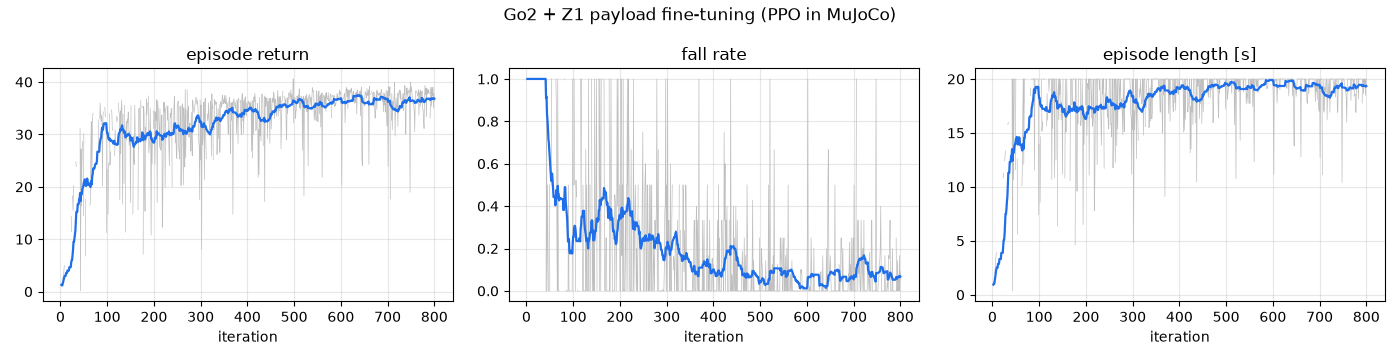
\includegraphics[width=\textwidth]{train_curve.png}\\[1pt]
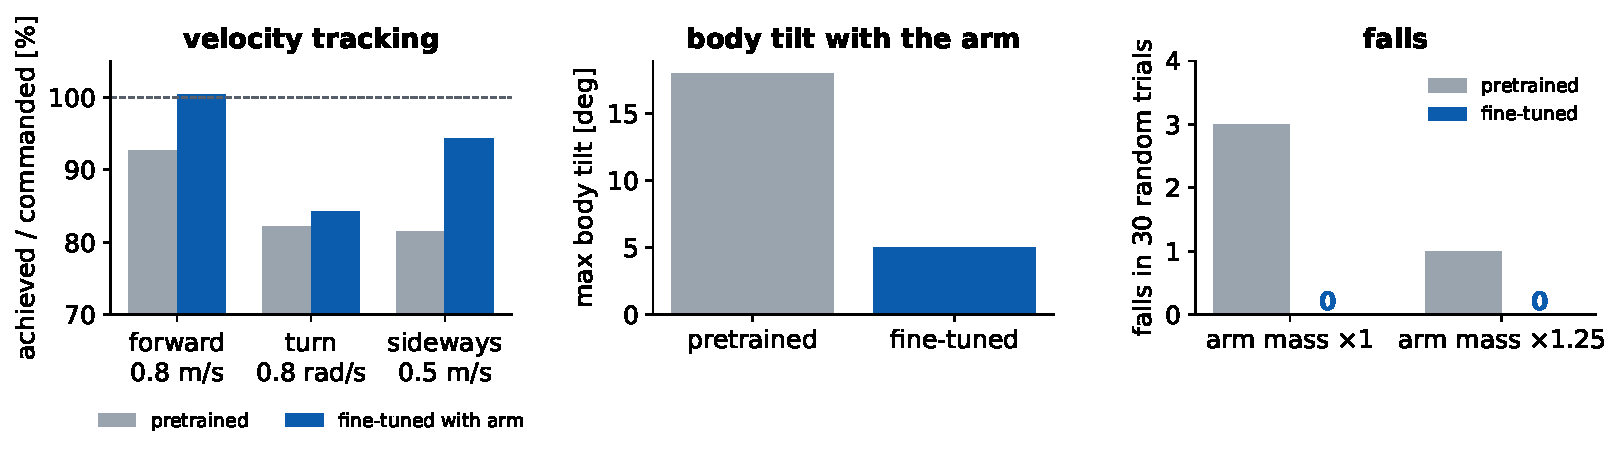
\includegraphics[width=\textwidth]{loco_finetune.pdf}
\end{columns}
\takeaway{Fine-tuned with the arm: falls 3/30 $\rightarrow$ 0/30, tilt 18$^\circ$ $\rightarrow$ 5$^\circ$. Stairs still use the blind MoE policy (flat-ground training).}
\end{frame}

% ================================================================== 6 WBC
\begin{frame}{Holding still while the arm works: the stance WBC as a QP}
\begin{columns}[c]
\column{0.6\textwidth}
\footnotesize Solved every 2\,ms (DAQP, $\approx$0.2\,ms):
\begin{align*}
\min_{\ddot q,\,f}\ & \textstyle\sum_i w_i\big\|J_i\ddot q + \dot J_i\dot q - a_i^\ast\big\|^2,\quad a_i^\ast = K_p e_i + K_d\dot e_i\\
\text{s.t.}\ & M_b\ddot q + h_b = J_{c,b}^{\top} f \hspace{1.95cm}\text{floating base}\\
 & J_c\ddot q + \dot J_c\dot q = -k_c J_c\dot q \hspace{1.05cm}\text{feet fixed}\\
 & |f_{x,y}|\le\mu f_z,\ f_z\ge 5\,\text{N} \hspace{1.35cm}\text{friction, }\mu{=}0.6\\
 & |\tau|\le\tau_{\max},\ \tau = M_a\ddot q + h_a - J_{c,a}^{\top}f
\end{align*}
\begin{itemize}\scriptsize
\item tasks $i$: rigid base, tool pose (+ clamped integral), arm posture
\item Z1 joint friction (1\,Nm): feed-forward on planned motion, or disturbance observer while tracking
\end{itemize}
\column{0.38\textwidth}
\centering
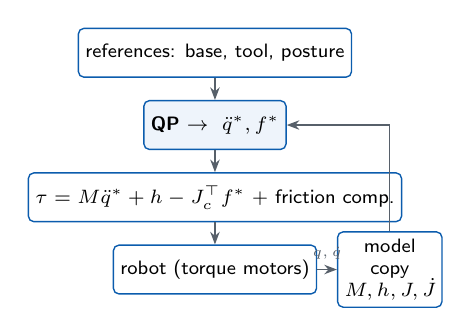
\begin{tikzpicture}[node distance=0.28cm]
\node[box] (ref) {references: base, tool, posture};
\node[hbox,below=of ref] (qp) {\textbf{QP} $\rightarrow\ \ddot q^\ast, f^\ast$};
\node[box,below=of qp] (id) {$\tau = M\ddot q^\ast + h - J_c^\top f^\ast$ + friction comp.};
\node[box,below=of id] (pl) {robot (torque motors)};
\node[box,right=0.25cm of pl,text width=1.15cm] (mod) {model copy\\$M,h,J,\dot J$};
\draw[arr] (ref)--(qp); \draw[arr] (qp)--(id); \draw[arr] (id)--(pl);
\draw[arr] (pl)--node[note,above]{$q,\dot q$}(mod);
\draw[arr] (mod.north) |- (qp.east);
\end{tikzpicture}
\end{columns}
\takeaway{Dynamics, contacts, friction and torque limits are hard constraints: the body moves 0.4\,mm while the tool tracks to 0.08\,mm (Go2).}
\end{frame}

% ================================================================== 7 hand-off + force
\begin{frame}{Pressing just right: hand-off and force control}
\begin{columns}[t]
\column{0.5\textwidth}
\textbf{\small Hand-off}\\[2pt]
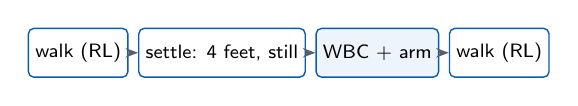
\begin{tikzpicture}[node distance=0.12cm]
\node[box] (a) {walk (RL)};
\node[box,right=of a] (b) {settle: 4 feet, still};
\node[hbox,right=of b] (c) {WBC + arm};
\node[box,right=of c] (d) {walk (RL)};
\draw[arr] (a)--(b); \draw[arr] (b)--(c); \draw[arr] (c)--(d);
\end{tikzpicture}\\[5pt]
\textbf{\small Along the normal $n$}: admittance on the tool target
\[\dot\delta = k_a\,(F^\ast - F),\qquad p_{\text{tool}} = p_{\text{surf}}(u,v) - \delta\,n\]
\textbf{\small Feed-forward}: $F^\ast n$ added to the WBC dynamics\\[3pt]
\textbf{\small Tangent plane}: raster + integral on the measured tip; tool axis $=$ measured normal
\column{0.48\textwidth}
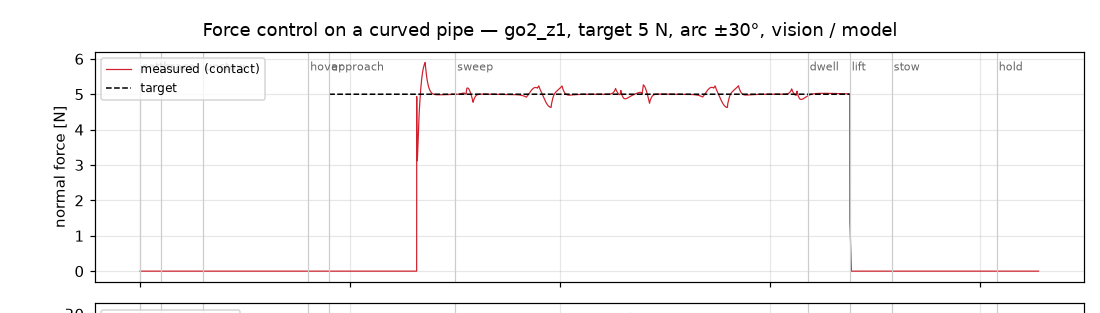
\includegraphics[width=\textwidth]{force_pipe_trace.png}\\[1pt]
\figcap{Pipe demo (force loop inside the QP), 5\,N over $\pm30^\circ$: 5.00\,N mean, 0.10\,N RMS, contact never lost, tool 0.34$^\circ$ from the real normal.}\vspace{3pt}
\scriptsize
\begin{tabular}{@{}lccc@{}}\toprule
vessel trace, feed-forward & mean & RMS err & peak\\\midrule
desired $F^\ast$ (used) & 5.01\,N & 0.28\,N & 6.2\,N\\
measured $F$ & 5.01\,N & 0.34\,N & 6.6\,N\\
none & 5.01\,N & 0.28\,N & 6.2\,N\\\bottomrule
\end{tabular}
\end{columns}
\takeaway{The admittance loop does the work: desired, measured or no feed-forward all hold 5.01\,N on the vessel (tested, same start).}
\end{frame}

% ================================================================== 8 perception + reach
\begin{frame}{From depth points to a surface model to a reach plan}
\centering
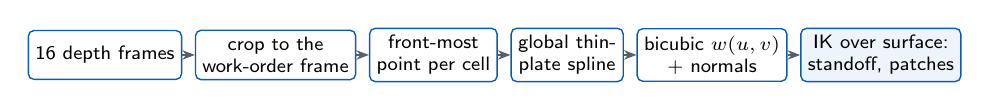
\begin{tikzpicture}[node distance=0.16cm]
\node[box] (p1) {16 depth frames};
\node[box,right=of p1] (p2) {crop to the\\work-order frame};
\node[box,right=of p2] (p3) {front-most\\point per cell};
\node[box,right=of p3] (p4) {global thin-\\plate spline};
\node[box,right=of p4] (p5) {bicubic $w(u,v)$\\+ normals};
\node[hbox,right=of p5] (p6) {IK over surface:\\standoff, patches};
\foreach \a/\b in {p1/p2,p2/p3,p3/p4,p4/p5,p5/p6} \draw[arr] (\a)--(\b);
\end{tikzpicture}\\[3pt]
\begin{columns}[t]
\column{0.52\textwidth}
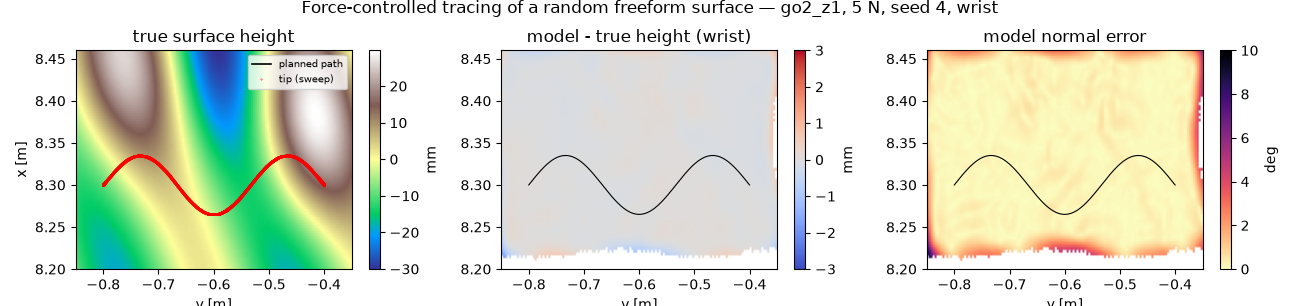
\includegraphics[width=\textwidth]{surface_model.png}\\
\figcap{Freeform-panel demo (wrist camera): model within 0.03--0.05\,mm and 0.2$^\circ$ along the path. Final mission (head camera): 0.1--0.2\,mm, 0.6--1.0$^\circ$ RMS.}
\column{0.46\textwidth}
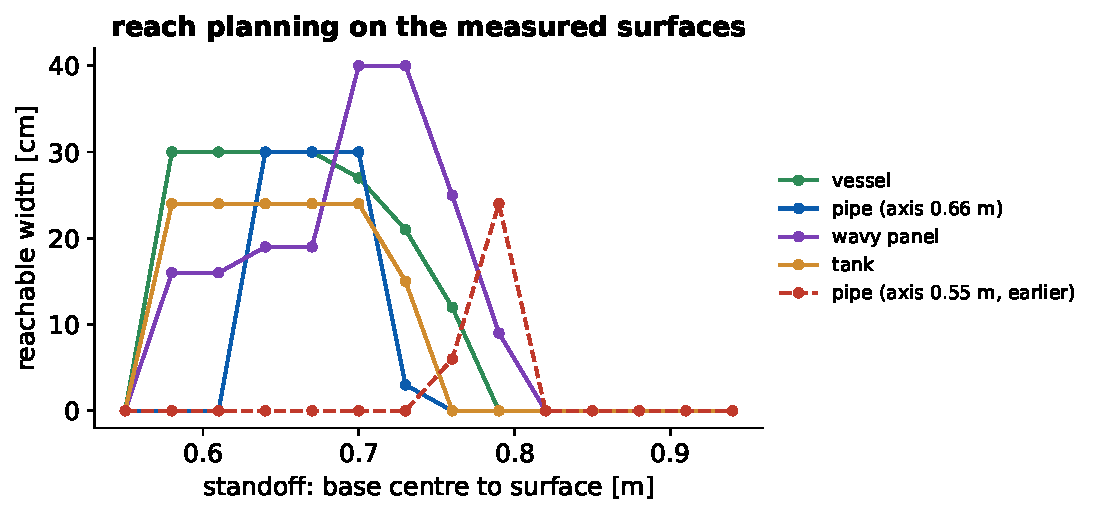
\includegraphics[width=\textwidth]{reach.pdf}\\
\figcap{Reachable width vs standoff (seed 3). Pipe axis at 0.55\,m: most of the strip from one standoff only; at 0.66\,m: the full strip from three.}
\end{columns}
\takeaway{No shape is assumed: one non-parametric model handles a vessel, a pipe, a tank and a random panel.}
\end{frame}

% ================================================================== 9 localisation + exploration
\begin{frame}{Where am I, and where to look next?}
\begin{columns}[t]
\column{0.42\textwidth}
\textbf{\small Localise}: match the depth scan to the map
\[\min_{\Delta x,\Delta y,\Delta\theta}\ \textstyle\sum_k \rho\big(\mathrm{SD}(R_{\Delta\theta}\,p_k + t)\big)\]
\begin{itemize}\scriptsize
\item SD = signed distance to map edges; Gauss--Newton, Huber $\rho$
\item only directions the scan constrains (eigenvalues of $J^\top J$)
\item partial-height objects ignored (pipe, tank, panel)
\end{itemize}
\textbf{\small Explore}: $\ v^\ast = \arg\max_v \text{unseen}(v)\cdot e^{-d(v)/6\,\text{m}}$
\begin{itemize}\scriptsize
\item seen = within 25$^\circ$ of the normal and 3.5\,m; A$^\ast$ on the grid, stairs = portal edge
\end{itemize}
\column{0.56\textwidth}
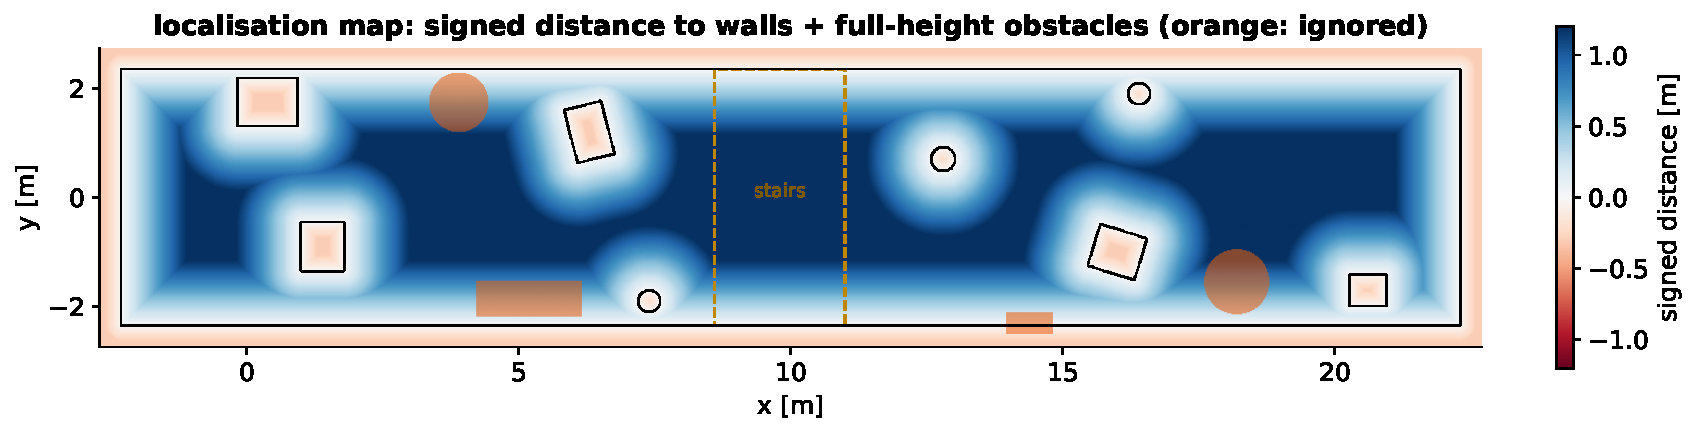
\includegraphics[width=0.85\textwidth]{sdf_map.pdf}\\[1pt]
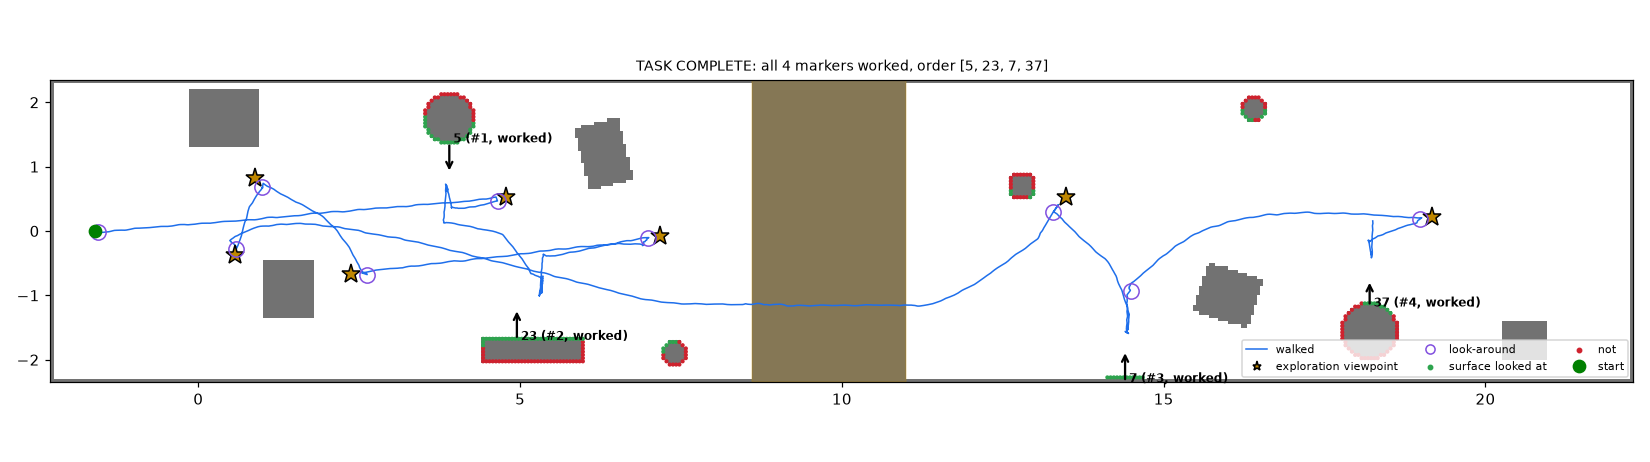
\includegraphics[width=0.85\textwidth]{explore_seed3.png}\\
\figcap{Seed 3: viewpoints (stars), look-arounds (circles), surfaces seen (green), markers in order worked.}
\end{columns}
\takeaway{The known map is enough: mean localisation error 0.8--1.8\,cm over whole missions, no SLAM.}
\end{frame}

% ================================================================== 10 setup + metrics
\begin{frame}{Experimental setup and metrics}
\begin{columns}[t]
\column{0.47\textwidth}
\textbf{\small Simulation}
\begin{itemize}\footnotesize
\item MuJoCo, 2\,ms physics; WBC 500\,Hz, policy 50\,Hz
\item torque motors, real limits (Go2 23.7/45.4\,Nm, Z1 30/60\,Nm)
\item 25 $\times$ 4.7\,m terrain corridor, full-width stairs, 4 surfaces
\end{itemize}
\textbf{\small Sensor models}
\begin{itemize}\footnotesize
\item RGB $1280{\times}720$; depth $160{\times}120$, noise $0.5\,\text{mm}+2\,\text{mm}\cdot z^2$
\item odometry: 3\,\% scale, 1\,\% yaw rate, 0.11$^\circ$/m
\item 3 noise seeds $\times$ 2 strategies
\end{itemize}
\column{0.51\textwidth}
\textbf{\small Metrics} (vs ground truth the robot never sees)\\[2pt]
\scriptsize
\begin{tabular}{@{}ll@{}}\toprule
coverage & share of the work area pressed\\
force & mean, RMS error, share in $5\,\text{N}\pm20\,\%$\\
contact lost & share of trace time with $F<0.5$\,N\\
dock error & true stance vs intended stance\\
localisation & estimate vs truth (position, heading)\\
time & robot time, distance walked\\\bottomrule
\end{tabular}
\end{columns}
\takeaway{Every number in the results comes from these runs and is checked against simulator ground truth.}
\end{frame}

% ================================================================== 11 results I
\begin{frame}{Results I: is the controller needed, and what does it need?}
\begin{columns}[t]
\column{0.47\textwidth}
\textbf{\small WBC vs baselines} {\scriptsize(precision task, Spot prototype)}\\[1pt]
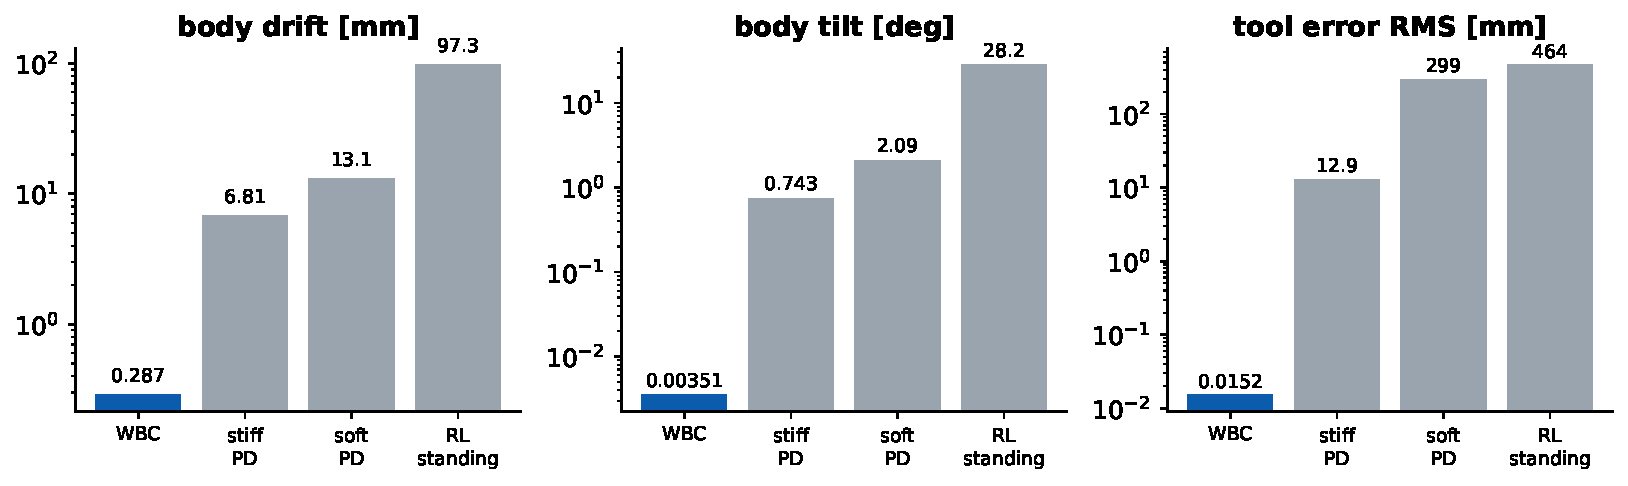
\includegraphics[width=\textwidth]{wbc_baselines.pdf}\\
\figcap{Log scale. Spot + arm + 1.2\,kg tool. Soft PD sags 227\,mm (seam out of reach); RL standing tilts 28$^\circ$. Same WBC on Go2: 0.40\,mm, 0.03$^\circ$, 0.08\,mm.}
\column{0.51\textwidth}
\textbf{\small Ablation} {\scriptsize(Go2; undo one choice at a time)}\\[1pt]
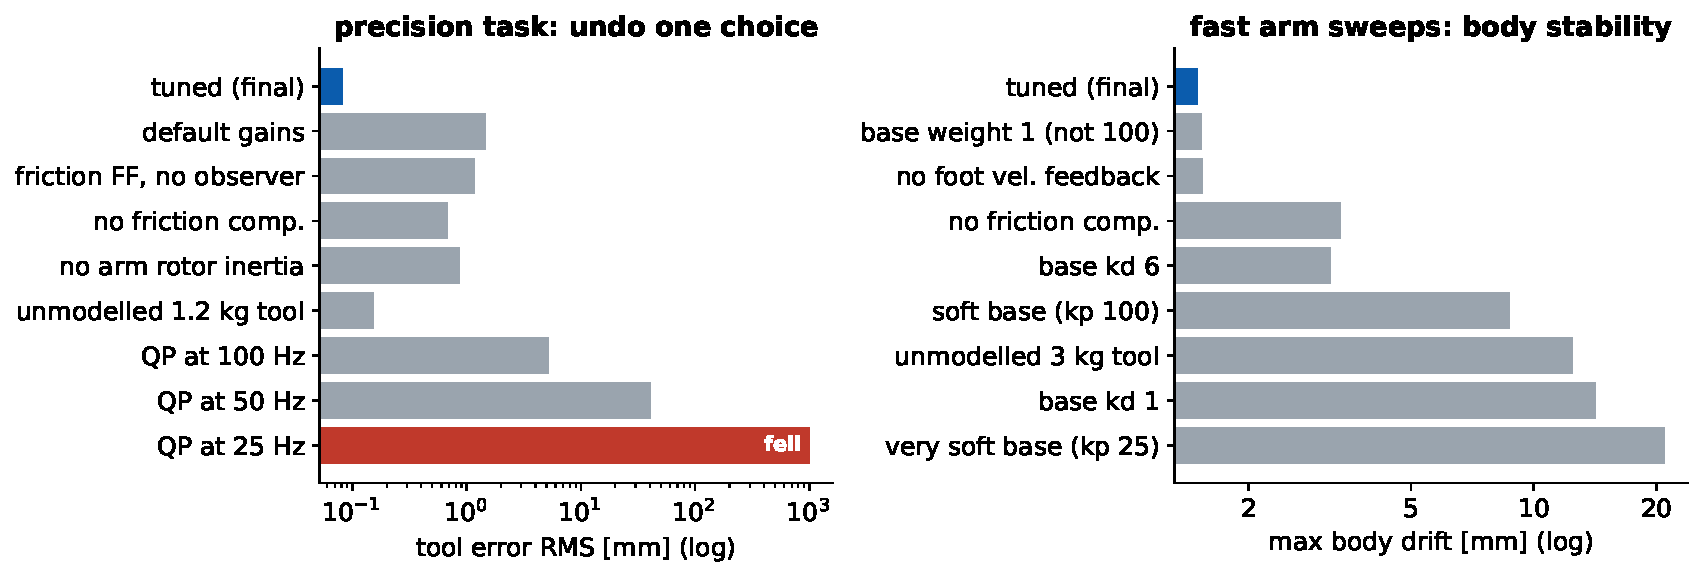
\includegraphics[width=\textwidth]{ablation.pdf}\\
\figcap{Control rate dominates (25\,Hz falls); friction handling and arm inertia matter at mm level; task weights barely matter.}
\end{columns}
\takeaway{24--850$\times$ better than stiff frozen legs on drift, tilt and tool error; control rate matters more than tuning weights.}
\end{frame}

% ================================================================== 12 results II
\begin{frame}{Results II: the full mission}
\begin{columns}[t]
\column{0.5\textwidth}
\tiny
\begin{tabular}{@{}lcccc@{}}\toprule
 & s1 & s2 & s3 & map first\\\midrule
complete & \checkmark & \checkmark & \checkmark & 3/3\\
time [s] & 696 & 731 & 705 & 730--775\\
coverage [\%] & 97--100 & 91--100 & 99--100 & 97--100\\
in $5\,\text{N}\pm20\%$ [\%] & 87--100 & 93--100 & 93--100 & 92--100\\
contact lost & 0 & 0 & 0 & 0\\
loc. error [cm] & 1.0 & 0.8 & 0.8 & 1.6--1.8\\\bottomrule
\end{tabular}\\[1pt]
\figcap{s1--s3: work as found, noise seeds 1--3; map first: seeds 1--3. Ranges over the 4 surfaces.}
\vspace{2pt}
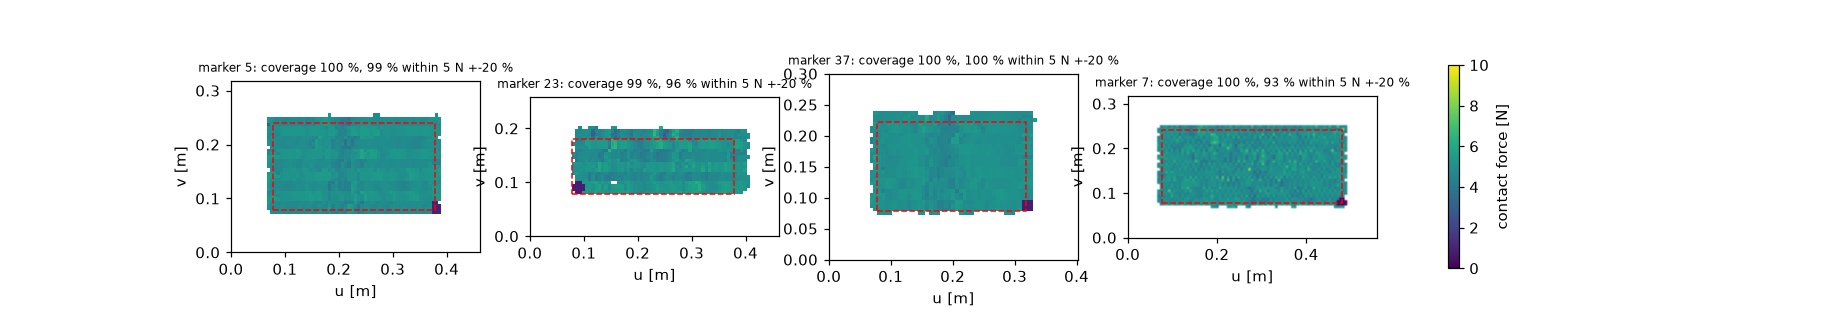
\includegraphics[width=0.95\textwidth]{paint_seed3.png}\\
\figcap{Seed 3: force applied over each area (dashed: work order).}
\column{0.48\textwidth}
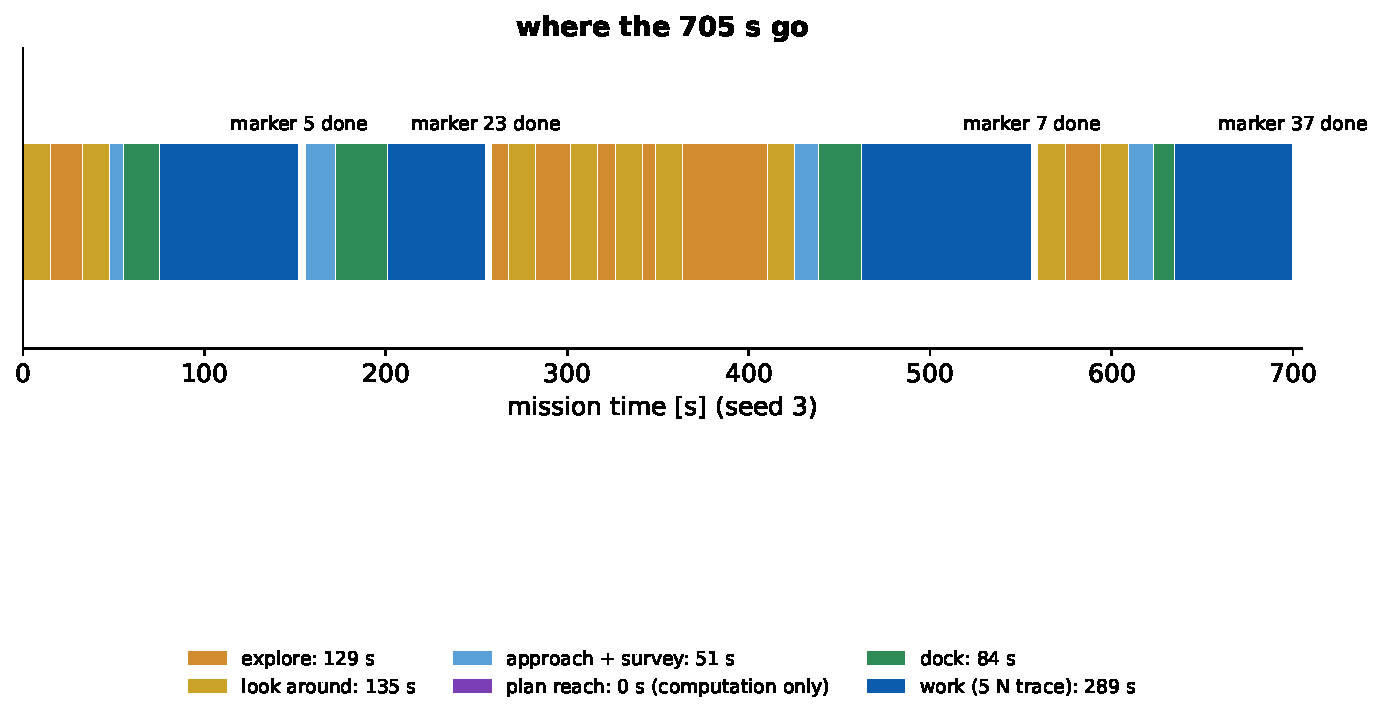
\includegraphics[width=\textwidth]{timeline.pdf}\\
\figcap{Seed 3, phases from the event log: tracing 41\,\%, exploring + looking around 37\,\%.}\vspace{3pt}
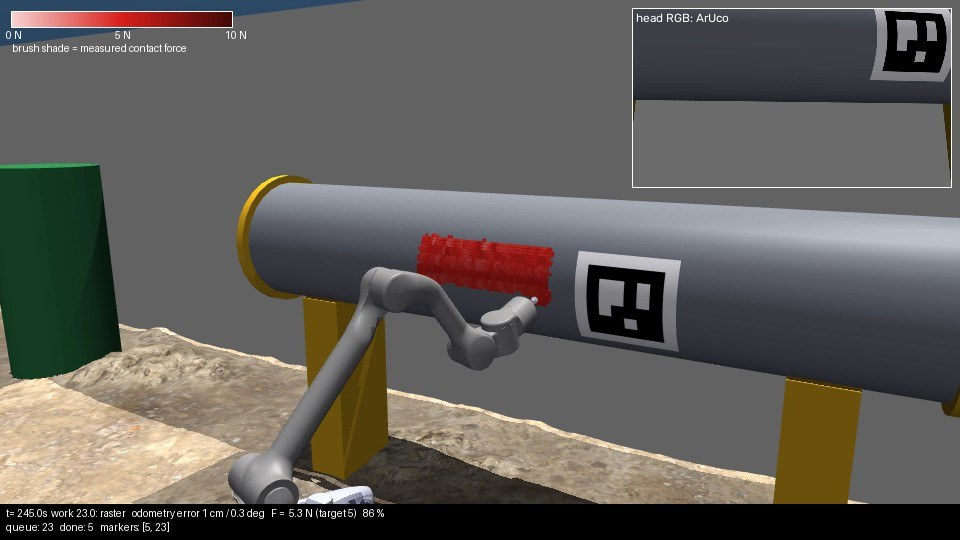
\includegraphics[width=0.49\textwidth]{final_pipe.jpg}\hfill
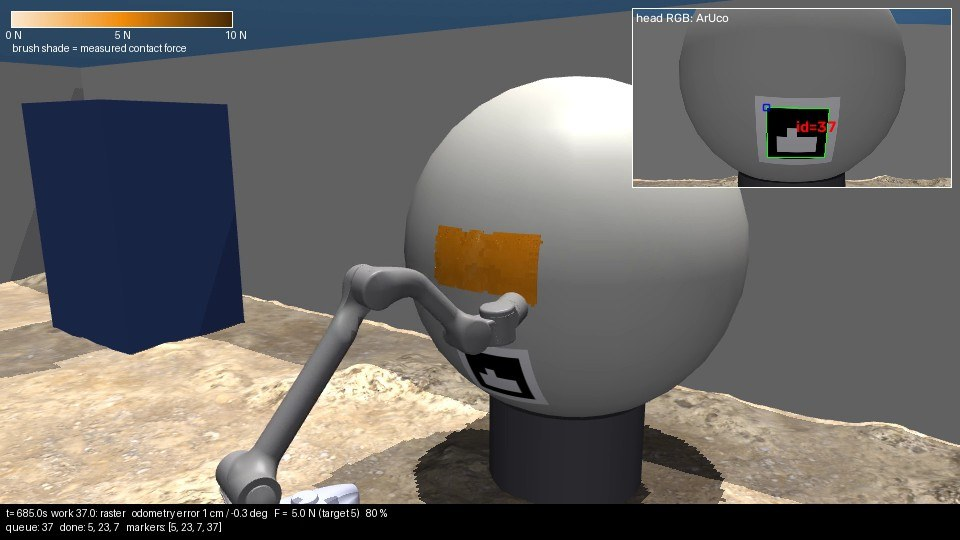
\includegraphics[width=0.49\textwidth]{final_tank.jpg}\\[1pt]
{\tiny\href{run:../../results/curved_mission/mission_seed3_video.mp4}{\color{accent}$\blacktriangleright$ video: results/curved\_mission/mission\_seed3\_video.mp4}}
\end{columns}
\takeaway{4 of 4 surfaces in all 6 runs (3 seeds $\times$ 2 strategies), 91--100\,\% covered at 5\,N, contact never lost.}
\end{frame}

% ================================================================== 13 compared with earlier
\begin{frame}{Why not the simpler versions? Compared with our earlier approaches}
\centering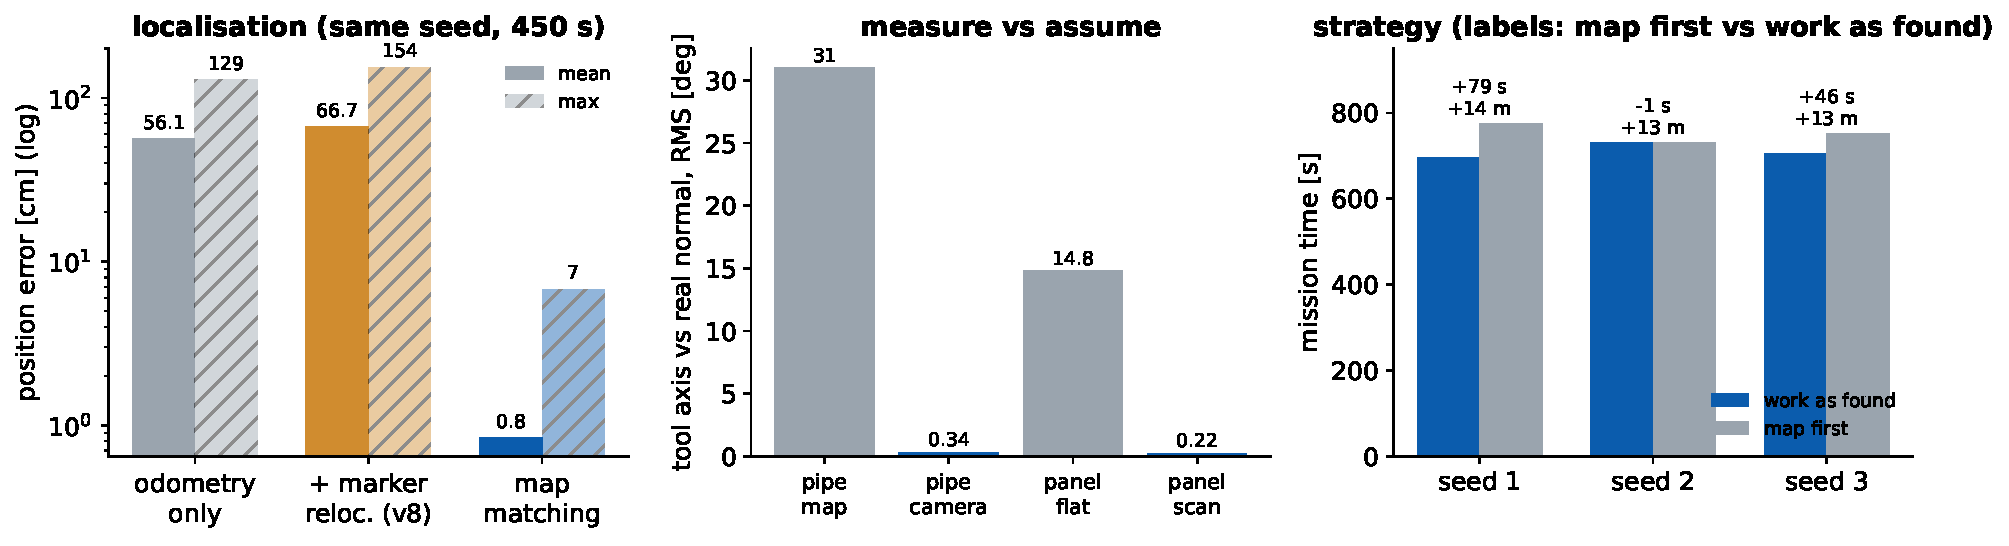
\includegraphics[width=0.8\textwidth]{before_after.pdf}\\[-1pt]\raggedright
\begin{columns}[t]
\column{0.46\textwidth}
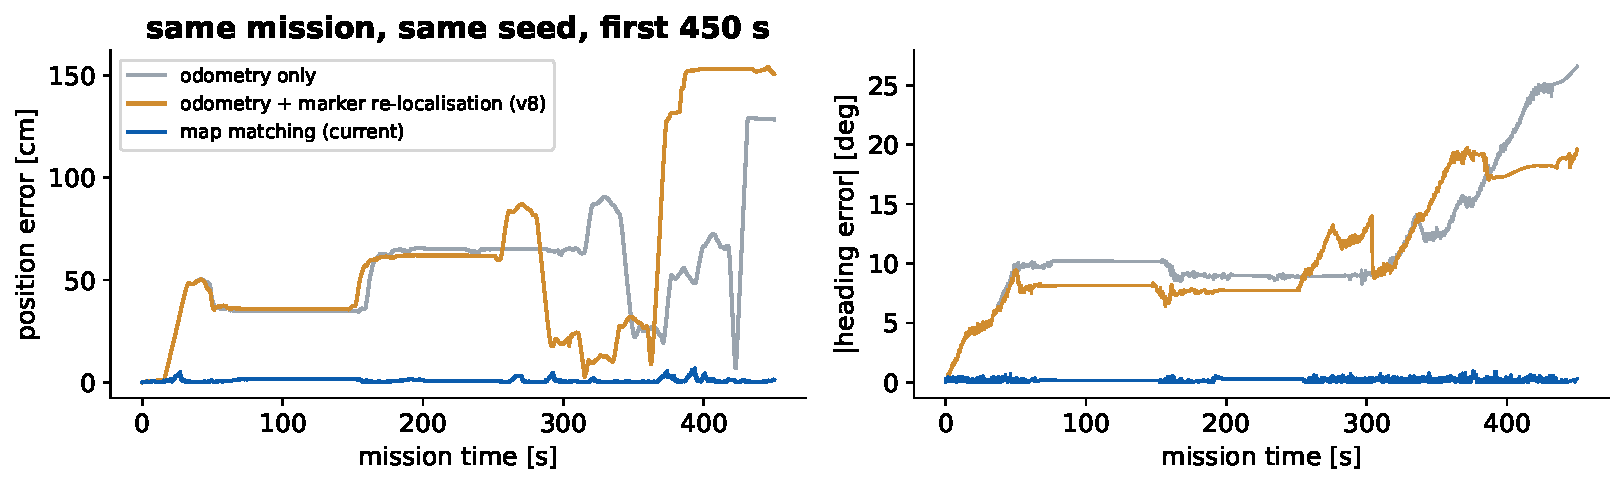
\includegraphics[width=0.92\textwidth]{loc_over_time.pdf}\\
\figcap{Same mission, same seed, first 450\,s; only the estimator changes. Map matching stays within 7\,cm and 1$^\circ$.}
\column{0.52\textwidth}
\begin{itemize}\tiny
\item \textbf{Robot}: Spot (no open stairs policy) $\rightarrow$ ANYmal (stairs needed GPU training) $\rightarrow$ Go2
\item \textbf{Localisation}: mean 56\,cm (odometry), 67\,cm (+ v8 marker re-localisation) $\rightarrow$ 0.8\,cm
\item \textbf{Perception}: assume $\rightarrow$ measure: tool angle 31$^\circ\rightarrow$0.3$^\circ$ (pipe), 14.8$^\circ\rightarrow$0.2$^\circ$ (panel)
\item \textbf{Strategy}: map first walks +13\,m every seed; time $-1$ to $+79$\,s; both complete
\end{itemize}
\end{columns}
\takeaway{Every simpler version was tried and measured; the re-localisation we started with was worse than odometry alone.}
\end{frame}

% ================================================================== 14 lessons + limits
\begin{frame}{Lessons learned and limitations}
\begin{columns}[t]
\column{0.48\textwidth}
\textbf{\small Lessons}
\begin{itemize}\footnotesize
\item Control rate before tuning: 500\,Hz works, 25\,Hz falls
\item Test what you believe: the force feed-forward we thought essential made no measurable difference
\item Curved stickers read at 30$^\circ$ off their normal, not at 45$^\circ$
\item 2-D footprints mislead scan matching near partial-height objects
\item Learned policies stop $\sim$5\,cm short: close the docking loop
\end{itemize}
\column{0.5\textwidth}
\textbf{\small Limitations}
\begin{itemize}\footnotesize
\item simulation only; the WBC reads the true state; the force sensor is ideal
\item tool = frictionless 8\,mm ball: contact force modelled, material removal not
\item no reaction to unmapped obstacles
\item pipe docks 5--10\,cm off (cause not isolated; absorbed by reach)
\item walking policy not trained with the arm on stairs
\end{itemize}
\textbf{\small Sim-to-real needs}: state estimation, filtered F/T sensing, a real tool and process model, a local obstacle layer
\end{columns}
\takeaway{Most of the work was finding out why things broke; the remaining gaps are known and listed.}
\end{frame}

% ================================================================== 15 conclusion
\begin{frame}{Conclusion and contributions}
\begin{columns}[t]
\column{0.56\textwidth}
\textbf{\small Contributions}
\begin{enumerate}\footnotesize
\item a \textbf{layered autonomy pipeline} for legged surface work: localise, decide, six-step execution, the same for every surface
\item \textbf{stance WBC + arm admittance}, with an ablation of what the controller needs
\item \textbf{map-matching localisation} and surface-model reach planning, evaluated over seeds and strategies
\end{enumerate}
\textbf{\small Built on}: pretrained Go2 policies (MoE-CTS), MuJoCo Menagerie models, a teammate's ArUco exploration mission
\column{0.42\textwidth}
\textbf{\small Next}
\begin{itemize}\footnotesize
\item local obstacle avoidance
\item a real grinding / inspection tool
\item walking fine-tuned with the arm on stairs
\item hardware transfer
\end{itemize}
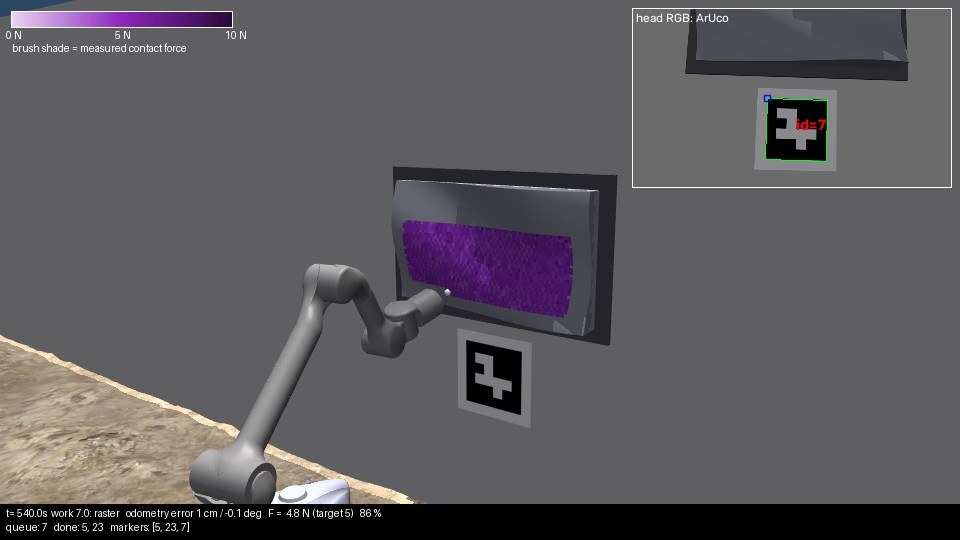
\includegraphics[width=0.85\textwidth]{final_panel.jpg}
\end{columns}
\takeaway{The robot finds, measures and treats unknown curved surfaces at 5\,N in every run; next it needs eyes for surprises and a real body.}
\end{frame}

% ================================================================== backup
\begin{frame}{Backup: full ablation table (Go2)}
\scriptsize\centering
\begin{tabular}{@{}lrrrrr@{}}\toprule
variant (precision task) & tool RMS [mm] & tool max [mm] & body drift [mm] & foot slip [mm] & peak torque\\\midrule
tuned (final) & 0.08 & 0.18 & 0.40 & 0.14 & 35\,\%\\
default gains & 1.46 & 3.18 & 0.43 & 0.14 & 35\,\%\\
no friction compensation & 0.69 & 1.81 & 1.01 & 0.17 & 36\,\%\\
friction FF, no observer & 1.16 & 1.98 & 0.47 & 0.14 & 35\,\%\\
no arm rotor inertia & 0.87 & 1.50 & 0.59 & 3.23 & 100\,\%\\
QP at 100 Hz & 5.22 & 8.91 & 3.53 & 213 & 100\,\%\\
QP at 50 Hz & 40.9 & 58.1 & 15.6 & 295 & 100\,\%\\
QP at 25 Hz & \multicolumn{5}{c}{fell}\\
unmodelled 1.2 kg tool & 0.15 & 0.35 & 1.06 & 0.81 & 77\,\%\\\bottomrule
\end{tabular}\\[8pt]
\begin{tabular}{@{}lrrrr@{}}\toprule
variant (fast arm sweeps) & body drift [mm] & tilt [deg] & speed RMS [mm/s] & foot slip [mm]\\\midrule
tuned (final) & 1.5 & 0.80 & 2.8 & 0.44\\
soft base (kp 100) & 8.7 & 3.18 & 7.6 & 1.07\\
very soft base (kp 25) & 20.9 & 5.41 & 11.6 & 1.77\\
base kd 1 & 14.2 & 3.92 & 97.1 & 55.9\\
unmodelled 3 kg tool & 12.5 & 0.80 & 16.6 & 50.6\\
base weight 1 / no foot vel. feedback & 1.5 & 0.80 & 2.9 & 0.45\\\bottomrule
\end{tabular}
\end{frame}

\begin{frame}{Backup: failure log (root cause $\rightarrow$ fix)}
\scriptsize\centering
\begin{tabular}{@{}lll@{}}\toprule
layer & failure & cause $\rightarrow$ fix\\\midrule
locomotion & Spot falls in arm sweeps, no stairs & no open policies $\rightarrow$ changed robot\\
locomotion & Go2 falls within 0.9\,s & wrong joint order $\rightarrow$ hips, thighs, calves\\
locomotion & turns at 0.22 of command & passive damping 4$\times$ training $\rightarrow$ matched\\
control & 3.6\,mm tool error & Z1 joint friction $\rightarrow$ feed-forward + observer\\
control & wrist roll runaway & no rotor inertia $\rightarrow$ 0.01\,kg\,m$^2$ armature\\
force & 36\,\% contact loss & friction FF ignored tool rotation $\rightarrow$ planned twist\\
perception & tip loses contact on a smooth panel & local RBF ripples $\rightarrow$ global spline\\
localisation & 1.1\,m / 14$^\circ$ drift (first version) & one-way turns, sparse markers $\rightarrow$ map matching\\
localisation & 26\,cm / 7.5$^\circ$ near the panel & partial-height footprints $\rightarrow$ excluded\\
exploration & tank marker never found & explorer angle 35$^\circ$ $\rightarrow$ 25$^\circ$\\
docking & stops 5\,cm short & policy settle $\rightarrow$ closed-loop dock correction\\
reach & pipe coverage 55--68\,\% & one feasible standoff $\rightarrow$ pipe at 0.66\,m\\
open & unmapped obstacle on the path & map-only planning $\rightarrow$ local obstacle layer (future)\\\bottomrule
\end{tabular}
\end{frame}

\end{document}
